\chapter{Monitorowanie klienta mobilnego}
\label{chap:Wymagania}

Współczesne systemy posiadają bardzo rozbudowane możliwości
monitorowania stanu infrastruktury złożonej z~urządzeń sieciowych,
stacji roboczych i~serwerów. Nowoczesne firmy posiadają jednak coraz
większe ilości sprzętu przenośnego, który również należy
monitorować. Wzrost liczby urządzeń mobilnych obecnych
w~infrastrukturach firm wynika nie tylko z~zakupów lecz także
z~popularyzacji podejścia BYOD czyli przynieś swoje własne urządzenie
(ang. {\em Bring Your Own Device}). W~firmach, które stosują to
podejście pracownicy upoważnieni są do przynoszenia do pracy swoich
prywatnych urządzeń, takich jak tablety, telefony czy
laptopy. Urządzenia te uzyskują dostęp do wielu chronionych zasobów
firmowych przez co konieczne jest zapewnienie w~organizacji
odpowiedniego poziomu bezpieczeństwa. Wraz z~popularyzacją rozwiązań
chmurowych pozwalających na realizację idei IaaS ({\em Infrastructure
  as a~Service}) możliwa jest tania i~wydajna wirtualizacja nie tylko
serwerów usługowych ale coraz częściej również stacji klienckich czy
całych aplikacji. Użytkownik może dzięki temu pracować w~tym samym
środowisku, niezależnie od urządzenia, które aktualnie
wykorzystuje. Zwiększa to elastyczność pracy, jednak niesie również za
sobą potrzebę monitorowania urządzeń mobilnych. W~przypadku urządzeń
firmowych pozwoli to np. na skorelowanie awarii występujących na
urządzeniach mobilnych, z~tymi, które występują na urządzeniach
stacjonarnych, oceny jakości urządzeń różnych producentów
itp. W~przypadku osób prywatnych monitoring urządzeń mobilnych może
służyć wykrywaniu zachowań potencjalnie niebezpiecznych lub kontroli
rodzicielskiej.  W~tym rozdziale przedstawiono charakterystykę
monitorowania klasycznej infrastruktury oraz takiej, w~której znajdują
się urządzenia mobilne. Ponieważ zagadnienie monitorowania tych
ostatnich jest rozwijane od niedawna, konieczna jest również definicja
wymagań stawianych tego typu systemom.

\section[Monitorowanie rozproszone][Monitorowanie rozproszone klientów
statycznych]{Monitorowanie rozproszone klientów statycznych}

Poprzez klienta statycznego rozumiemy wszelkie urządzenia stacjonarne
wchodzące w~skład infrastruktury IT przedsiębiorstwa, które pracują
nieprzerwanie lub w~dobrze określonych przedziałach czasowych
i~posiadają dobrze zdefiniowaną hierarchię. Wzajemne relacje pomiędzy
tymi urządzeniami wynikają w~dużej mierze ze~struktury sieci, lecz
mogą wynikać także z~roli, jaką odgrywają w~danej
organizacji. Przykładem klienta statycznego mogą zarówno serwery oraz
stacje robocze, jak i~routery lub urządzenia montażowe przy taśmie
produkcyjnej. Dzięki monitorowaniu wszystkich urządzeń w~danej sieci
systemy monitorujące są w~stanie wspierać administratora, wskazując
z~bardzo dużym prawdopodobieństwem miejsce wystąpienia awarii.

Cechą charakterystyczną systemów monitorowania klienta statycznego
jest operowanie zawsze na aktualnych danych. Urządzenie posiadają
stałą łączność pomiędzy sobie dlatego wszystkie wyniki sprawdzeń mogą
być na bieżąco przetwarzane przez system monitorujący. Każde zerwanie
łączności oznacza sytuację awaryjną, która musi być raportowana
użytkownikowi.

\begin{figure}[ht]
  \caption{Monitoring pasywny (schemat po lewej) oraz rozproszony
    (schemat po prawej). Kolor czerwony --- monitorowanie aktywne,
    niebieski --- monitorowanie pasywne, czarny --- komunikacja wewnętrzna
    systemu.}
  \label{fig:PorPasIRozp}
\makebox[\textwidth]{%
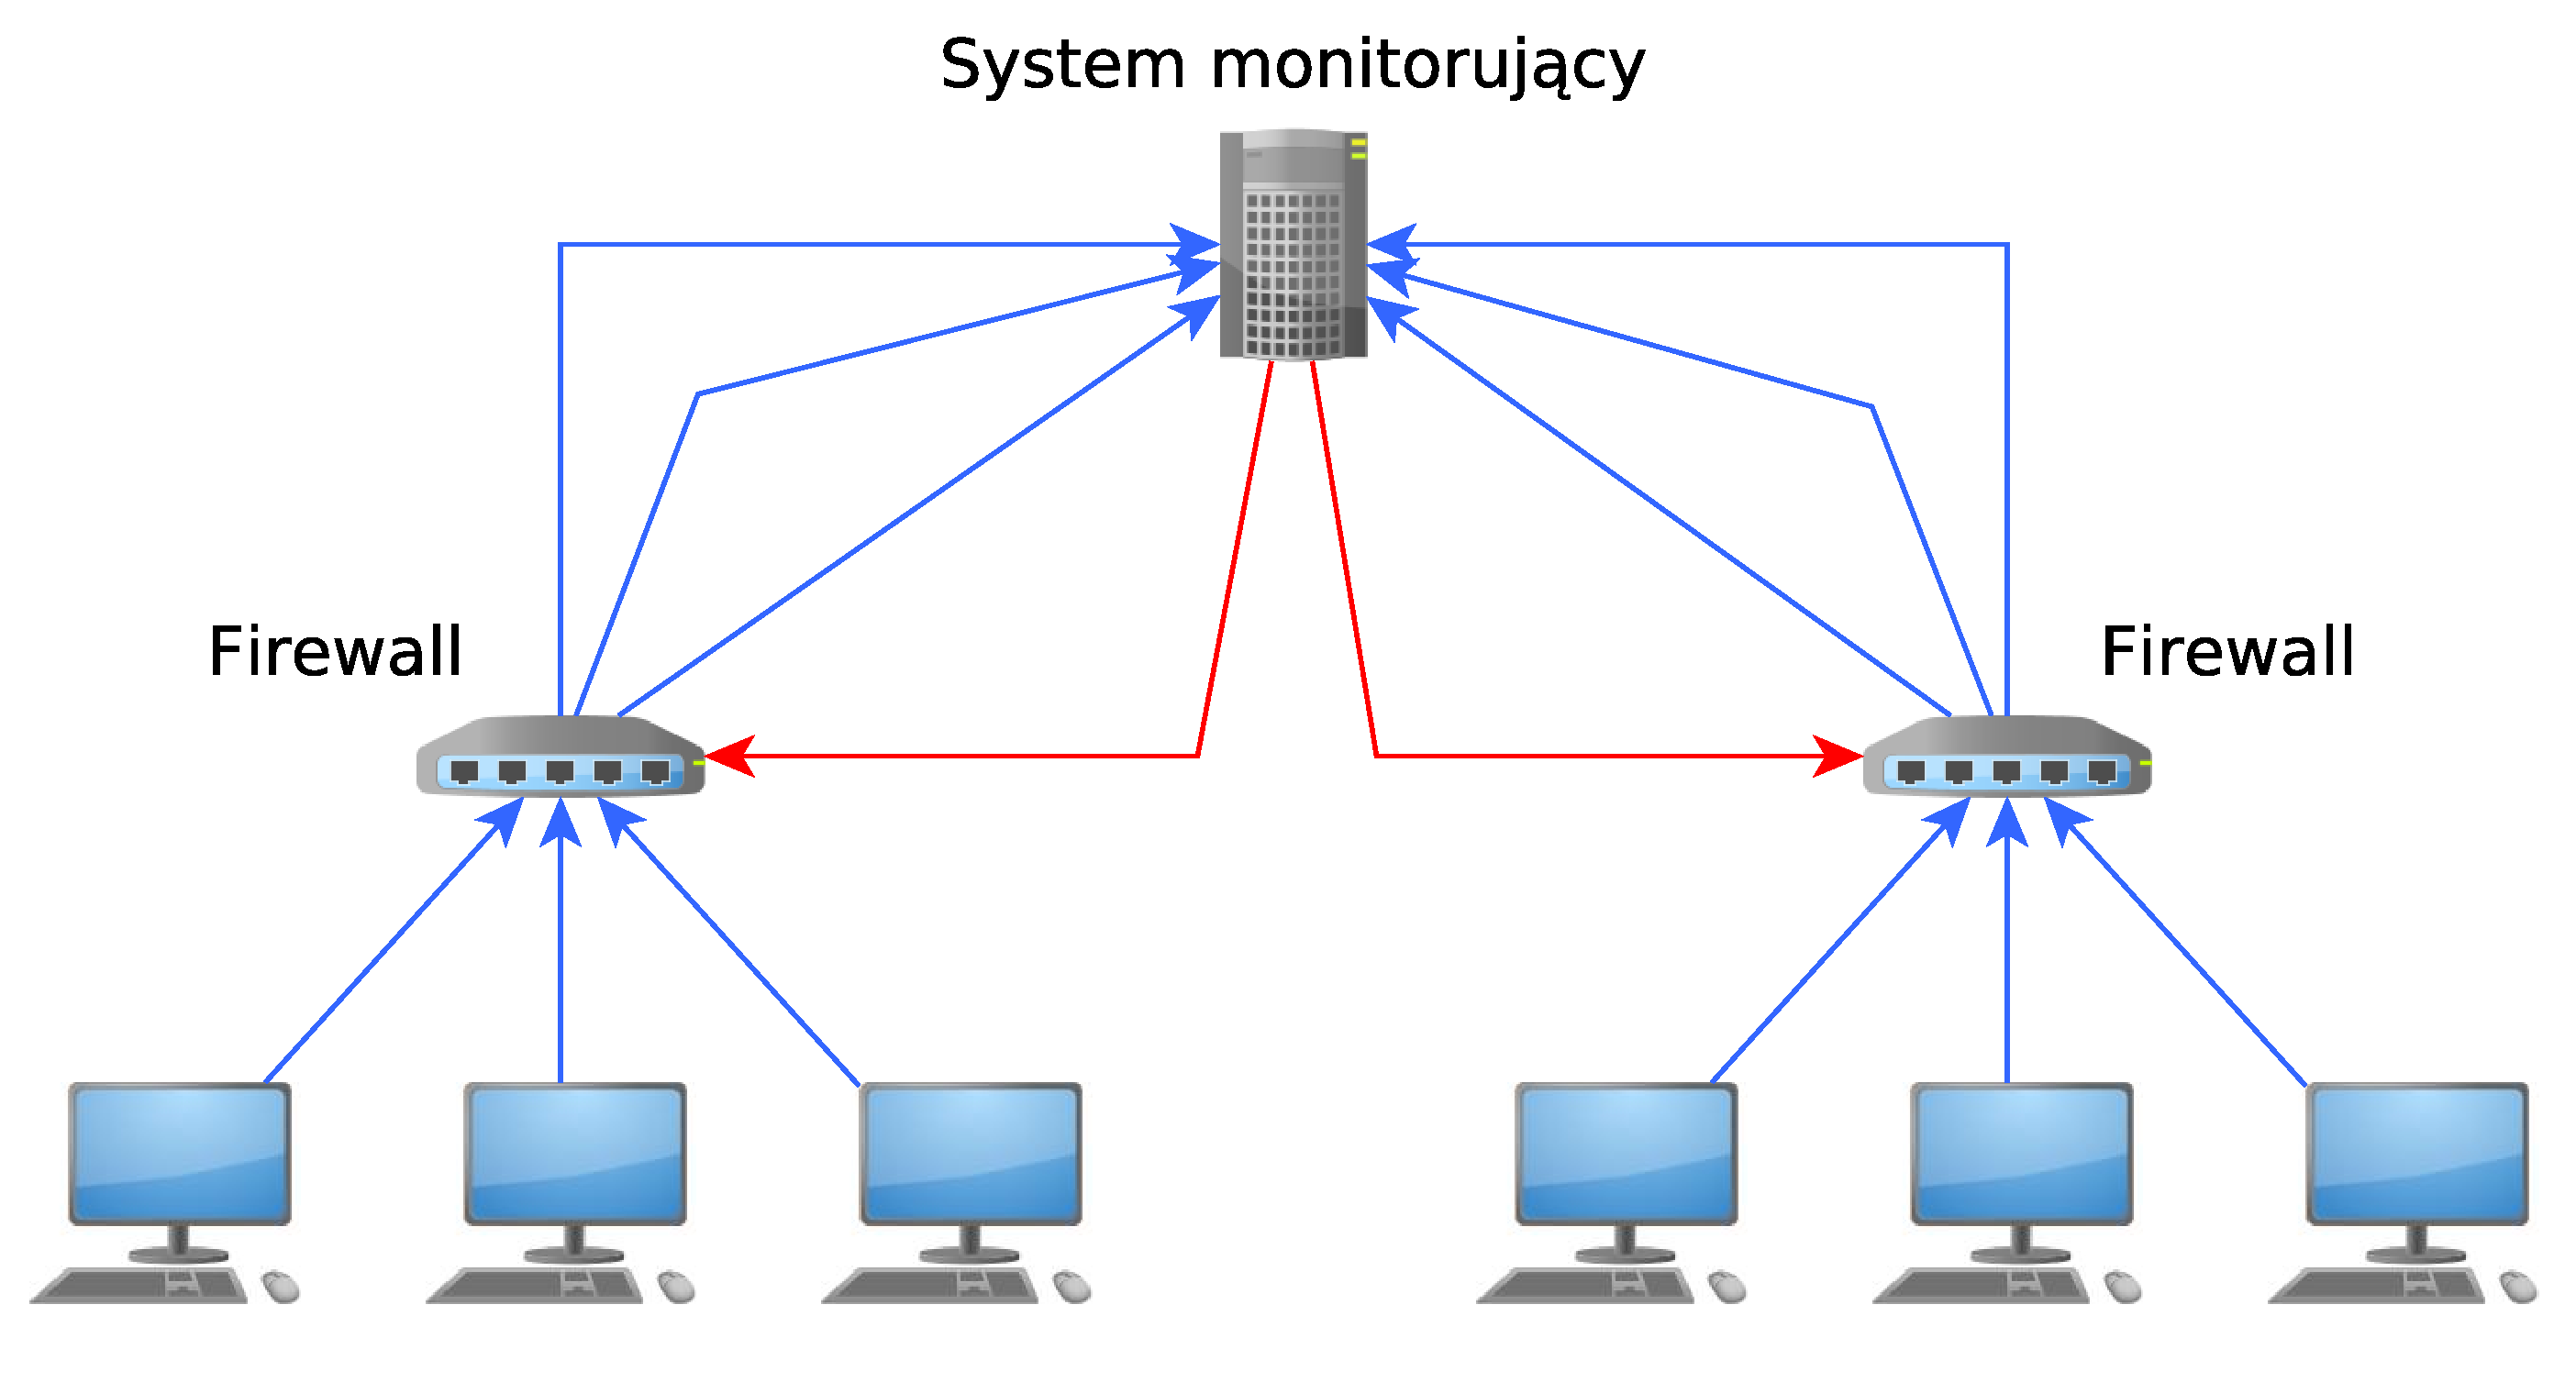
\includegraphics[width=0.49\textwidth]{img/pasywne}
\hfill    
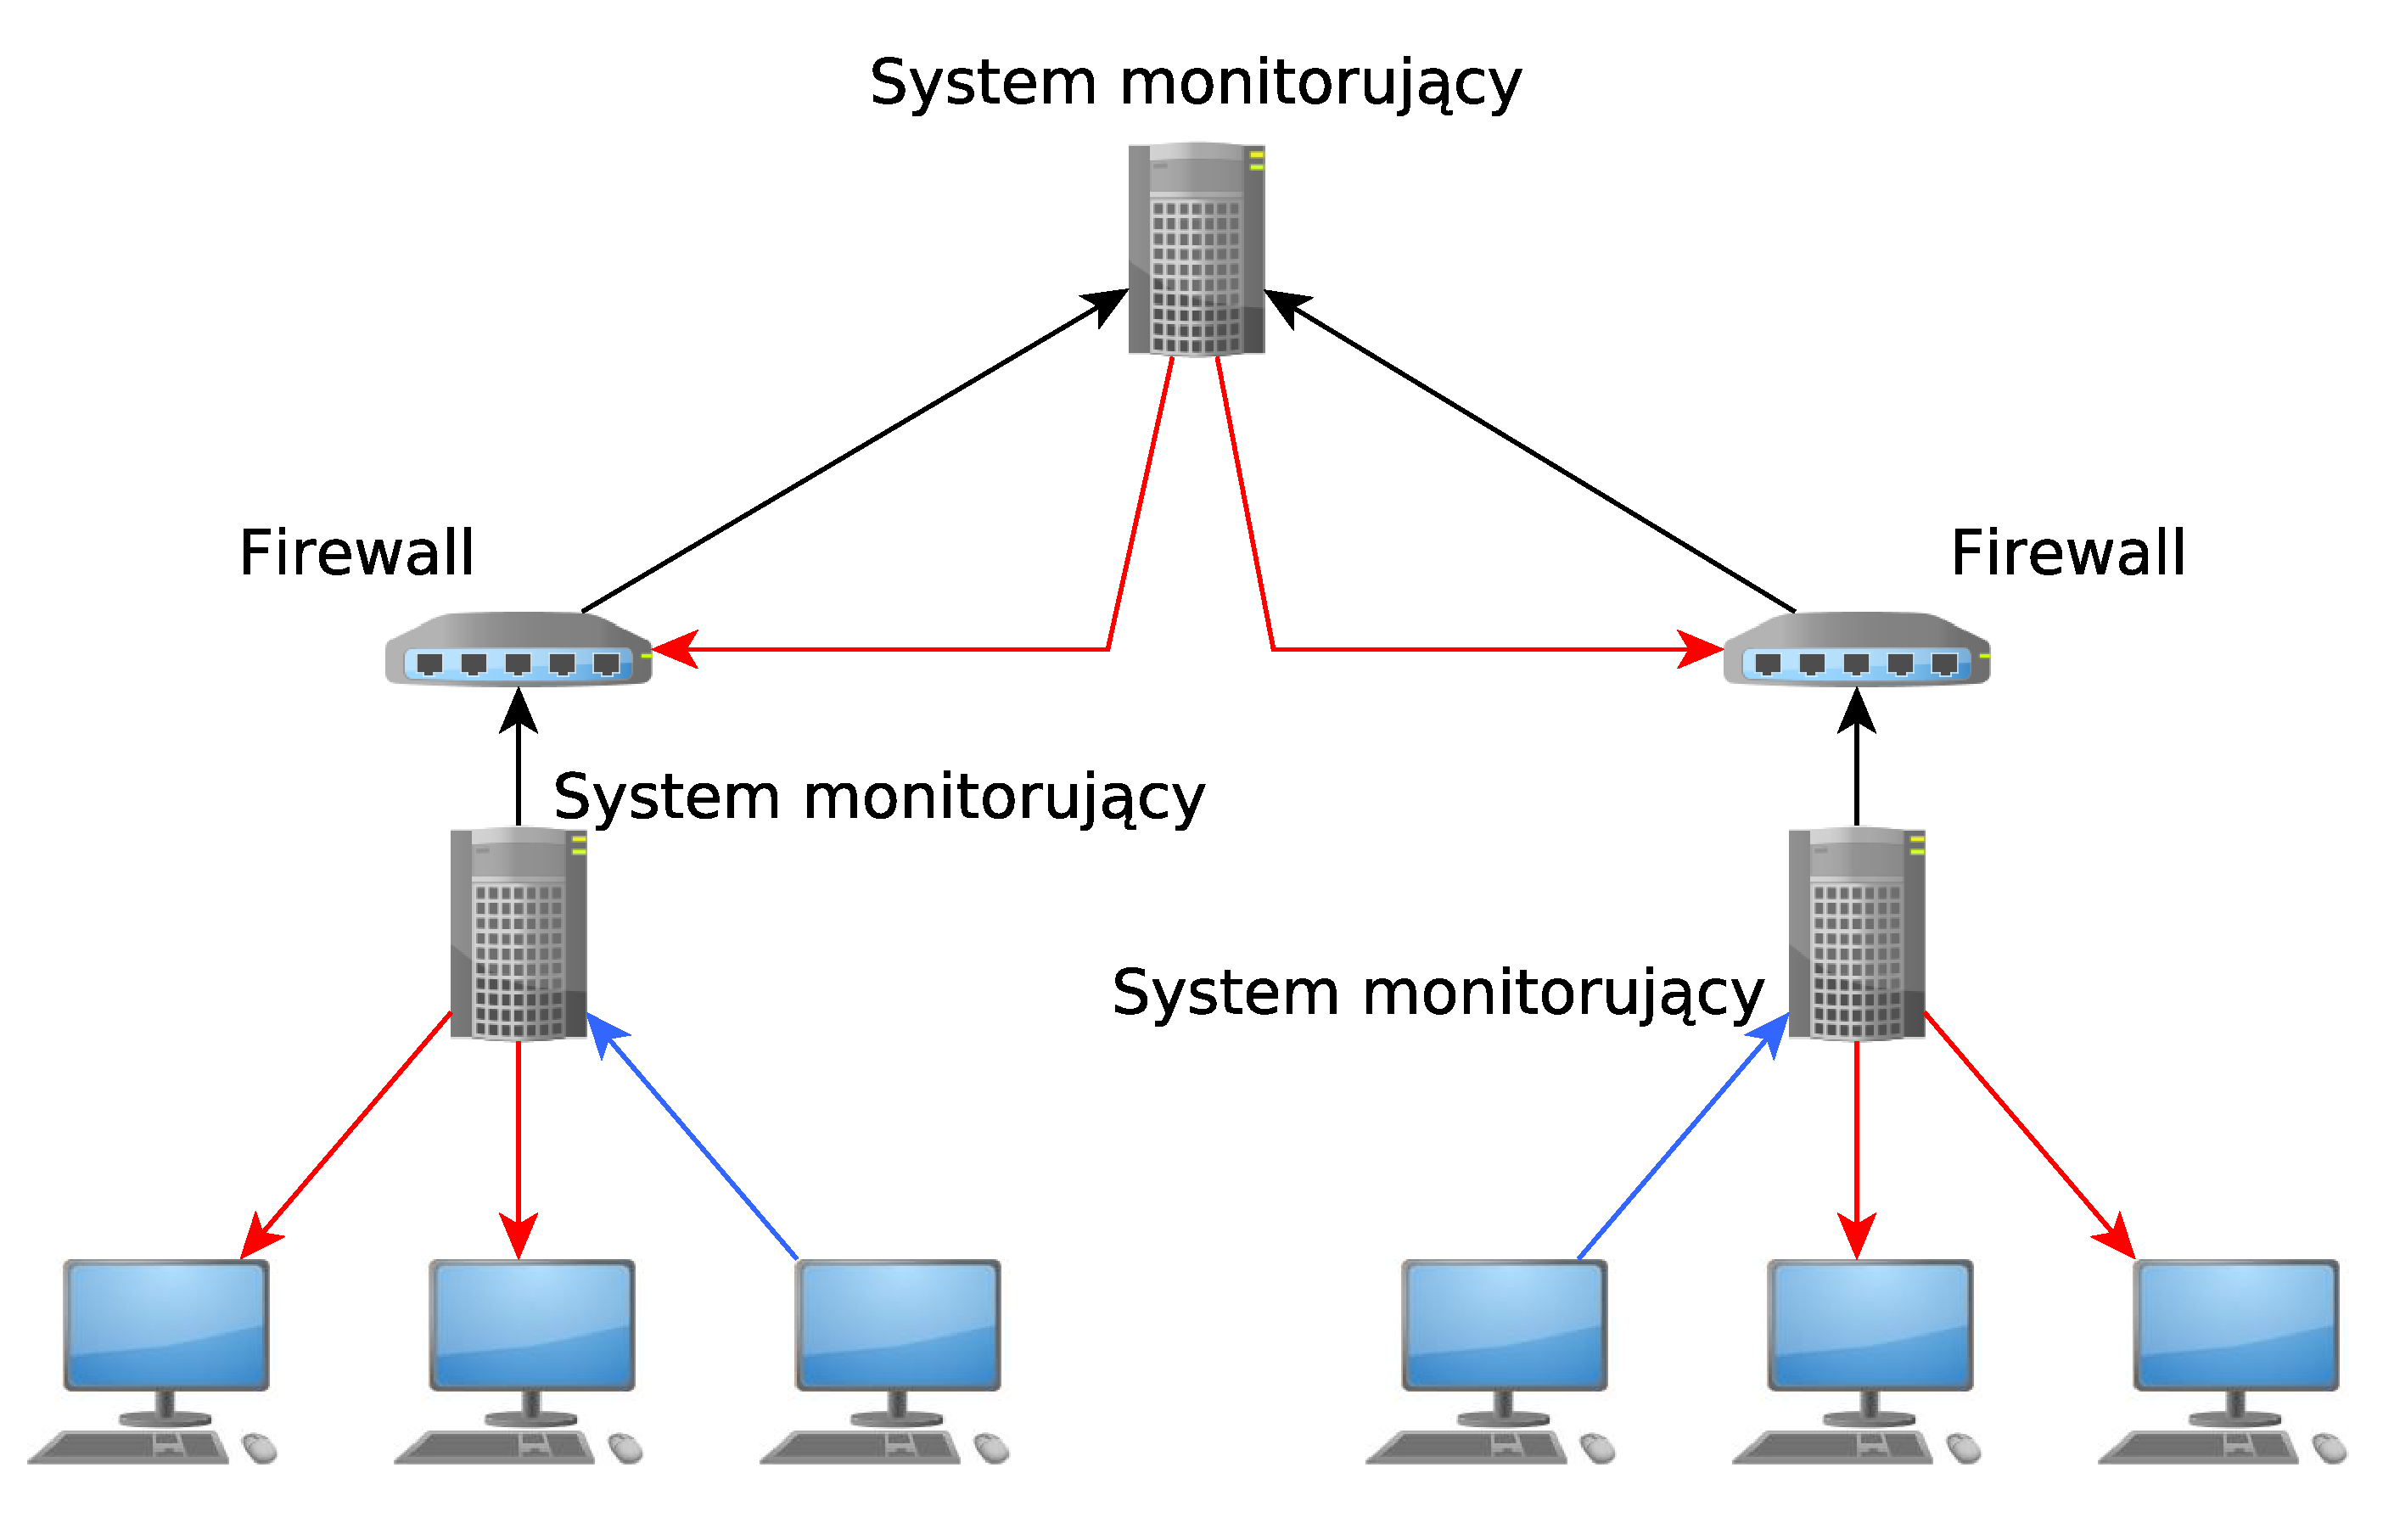
\includegraphics[width=0.49\textwidth]{img/rozproszone}
}\\[0.1cm]
\end{figure}

Sieć w~dużej firmie rzadko stanowi jedną całość. Zazwyczaj są to
segmenty sieci VLAN oddzielone zaporami lub w~ogóle wydzielone
fizycznie sieci LAN. Taka separacja urządzeń pozwala na zwiększenie
poziomu bezpieczeństwa, lecz jednocześnie utrudnia monitorowanie całej
infrastruktury. W~celu umożliwienia monitorowania całej sieci firmowej
wykorzystuje się monitorowanie rozproszone. Można wyróżnić dwie
podstawowe konfiguracje monitorowania rozproszonego (patrz
rys.~\ref{fig:PorPasIRozp}):

\begin{description}
\item[Monitorowanie pasywne] --- istnieje jedna, centralna instancja
  rdzenia monitorującego, do którego przesyłane są wyniki sprawdzeń
  poszczególnych usług. Każde urządzenie samo monitoruje swoje usługi
  i~zgłasza rezultaty.
\item[Wieloinstancyjny system monitorujący] --- istnieje wiele
  instancji rdzenia monitorującego. Typowo, każda wydzielona część
  sieci posiada swoją instancję. Każda instancja może posiadać zarówno
  usługi monitorowane aktywnie, jak i~pasywnie. Wyniki sprawdzeń
  przesyłane są następnie do jednej wybranej instancji, która gromadzi
  wszystkie dane lub centralnej bazy danych.
\end{description}

Użycie monitorowania pasywnego dla wszystkich usług jest bardzo
niewygodne i~jednocześnie utrudnia konfigurację, a~także pozbawia
administratora możliwości używania niektórych mechanizmów dostępnych
wyłącznie dla urządzeń monitorowanych aktywnie. Przykładem takiego
mechanizmu może być adaptacyjna częstotliwość wykonywania pomiarów
w~zależności od zmienności stanu urządzenia. Ponadto wyniki sprawdzeń
pasywnych typowo nie są buforowane, lecz wysyłane od razu po ich
uzyskaniu. Oznacza to, że jeśli pojawi się chwilowy brak połączenia
z~serwerem, to dane pomiarów zostaną utracone. W~przypadku, gdy
jedynym celem systemu jest monitorowanie dostępności danej usługi
zewnętrznej serwera, a~nie jego parametrów wewnętrznych, jest to jednak
błąd pomijalny. Błąd ten staje się jednak istotny, gdy jednym z~zadań
systemu jest gromadzenie i~analiza danych historycznych.

Wieloinstancyjny system monitorujący wymaga zdecydowanie więcej
zasobów, jednak pozwala na osiągnięcie znacznie wygodniejszego
i~bardziej niezawodnego systemu. Ponadto dzięki takiej konfiguracji
nie ma potrzeby ingerencji w~monitorowane serwery, gdyż możliwe jest
monitorowanie ich usług w sposób aktywny. Redukuje to ich obciążenie,
a~także zwiększa bezpieczeństwo. Warto również wspomnieć, że na
przykład system {\em Icinga} daje możliwość integracji wielu instancji
rdzenia monitorującego przy pomocy wspólnej bazy danych. Dzięki temu
administrator danej sieci ma możliwość monitorowania i~konfigurowania
wielu instancji przy pomocy wspólnego interfejsu. Niestety, w~systemie
Nagios rozwiązanie to zaliczane jest do części korporacyjnej tego
systemu, przez co posiada zamknięte źródła i~jego wykorzystanie wymaga
zakupu licencji. Rozwiązania oparte na istnieniu jednej centralnej
instancji rdzenia systemu monitorującego są zazwyczaj
darmowe. Wymagają one dodatkowej instancji, zajmującej się agregacją
danych co powoduje zwiększenie zużycia zasobów. Należy również zwrócić
uwagę, iż niektóre systemy jak Cacti nie posiadają w~ogóle możliwości
monitorowania pasywnego czy rozproszonego.

\section[Monitorowanie rozproszone][Monitorowanie rozproszone klientów
mobilnych]{Monitorowanie rozproszone klientów mobilnych}

Rosnąca w~ostatnich latach popularność technologii mobilnych
przyczyniła się do pojawienia się w~firmach bardzo dużej liczby
urządzeń mobilnych, które również wymagają zarządzania
i~monitorowania. Urządzenia mobilne są używane bardzo często przez
przedstawicieli handlowych oraz menadżerów w~celu wykonywania pracy
poza obszarem firmy. Duże korporacje coraz częściej decydują się
również na wyposażenie swoich pracowników w~smartfony lub tablety,
które mają ułatwić współpracę z~firmą w trakcie podróży służbowych czy
spotkań z~klientami.

Klient mobilny posiada szereg cech, które znacząco odróżniają go od
klientów statycznych. Przede wszystkim należy zauważyć, że urządzenia
o~których mowa, bardzo często pracują poza obszarem firmy. Wynika
z~tego, że nie zawsze możliwe jest utrzymywanie takich urządzeń
w~wirtualnej sieci prywatnej, gdyż urządzenie może znaleźć się
w~obszarze, gdzie w~ogóle nie ma dostępu do Internetu. Ponadto, nie
zawsze konieczne jest, aby urządzenia mobilne pracowały podłączone do
sieci firmowej. Użytkownicy często wymagają jedynie dostępu do
internetu i~innych funkcji tego urządzenia. Warto więc zauważyć, że
urządzenia te są często narażone na dostęp do sieci o~bardzo niskim
poziomie zaufania i~wielu zagrożeniach. Oznacza to w~szczególności, iż
urządzenie mobilne zazwyczaj posiada zmienny adres IP, który rzadko
jest adresem globalnym. Również struktura sieci, z~której korzystają
klienty mobilne jest dynamiczna i~znajduje się poza obszarem
monitorowania administratorów danego przedsiębiorstwa. Oznacza to, że
w~przeciwieństwie do klienta statycznego, gdzie każda utrata łączności
była awarią, utrata łączności jest normalnym elementem działania
systemu. Stwarza to konieczność okresowego gromadzenia danych
bezpośrednio na urządzeniu mobilnym oraz ich odsyłania w~dogodnym
czasie.

Znacząca większość klientów mobilnych dzięki kontaktom z~siecią
pozafirmową posiada, w~przeciwieństwie do klientów statycznych,
możliwość synchronizacji swojego czasu czy to z~serwerami czasu
światowego, czy też z~sieci GSM. Znaczne rozsynchronizowanie zegarów
urządzenia mobilnego z~urządzeniami w~firmie prowadzić może do
istotnych problemów funkcjonalnych (np. brak możliwości
uwierzytelnienia, trudność w śledzeniu kolejności zdarzeń). Warto
jednak przyjąć pewne określone zakresy tolerancji czasowych. Wśród
serwerów czas jest synchronizowany z~dokładnością do milisekund. Taka
dokładność w~przypadku klienta mobilnego jest zazwyczaj
zbędna. Bardzo często istotnymi jednostkami czasu stają się dopiero
sekundy lub nawet minuty.

Należy również zwrócić uwagę na duże rozproszenie klientów
mobilnych. W~przeciwieństwie do klientów statycznych, którzy zazwyczaj
pracują w~pewnych grupach lub fragmentach sieci, klienty mobilne są
zazwyczaj rozpatrywane pojedynczo. Większość klientów mobilnych
operuje w~pełni samodzielnie, zatem liczność grupy klientów
wynosi~1. Istnieją jednak zastosowania, gdzie jeden pracownik użytkuje
pewien niewielki zestaw urządzeń przenośnych. Nie zmienia to jednak
faktu, że grupa urządzeń mobilnych posiada liczność rzędu maksymalnie
kilku urządzeń, a nie nawet do kilkuset jak w przypadku klientów
statycznych. W~przeciwieństwie do klientów statycznych, gdzie grup
koniecznych do wydzielenia było zazwyczaj kilka lub kilkanaście,
w~przypadku klientów mobilnych takich grup może być kilkaset lub nawet
kilka tysięcy.

Warto również dostrzec różnice w~sposobie zasilania. Klienty mobilne
zazwyczaj posiadają własne zasilanie, przez co każda wykonywana na nim
operacja nie tylko spowalnia jego działanie, lecz również zmniejsza
jego czas pracy pomiędzy ładowaniami. Przenośność klienta mobilnego
zmienia również jego stopień bezpieczeństwa. Urządzenia mobilne
stosunkowo często są gubione lub kradzione. W~związku z~możliwością
utraty urządzenia nie powinno się na nim przechowywać tajnych danych,
dzięki którym można by skompromitować cały system z~którego korzysta
klient.

Klient mobilny znacznie różni również zbiorem elementów elementów,
które są monitorowane. W~przypadku klientów statycznych znaczna część
wysiłków jest ukierunkowana na pomiar usług świadczonych przez dany
system na rzecz innych systemów lub systemów świadczących określone
usługi dla systemu klienckiego (pomiar jakości usługi z punktu
widzenia urządzenia klienckiego). Natomiast w~przypadku klientów
mobilnych istotniejsze wydaje się być monitorowanie parametrów
wewnętrznych danego klienta i~ewentualnie usług świadczonych przez
klienta w ramach grupy klientów mobilnych. Przykładem może być laptop
oraz telefon komórkowy, który pozwala mu na dostęp do
Internetu. Istotne z~punktu widzenia monitorowania są parametry
wewnętrzne obu tych urządzeń takie jak stan baterii, siła sygnału
itd. oraz jakość usługi --- w~tym przypadku usługi dostępu do
internetu świadczonej przez telefon na rzecz laptopa. Sytuacja ta jest
typowa i~nie jest zazwyczaj spotykane, aby klient mobilny udostępniał
swoje usługi poza grupę klientów, w~której on operuje.

\section[Wymagania][Wymagania dla systemu monitorowania]{Wymagania dla systemu monitorowania}

Klient mobilny posiada zdecydowanie odmienną charakterystykę niż
klient statyczny. Dokonano zatem analizy, jakie wymagania należy
spełnić, aby dostarczyć system, który sprosta oczekiwaniom
administratorów urządzeń mobilnych i~statycznych.

Odbiorcą systemu mają być duże firmy i~korporacje, które posiadają
bardzo rozbudowaną sieć wewnątrz firmy, a~ponadto udostępniają swoim
pracownikom urządzenia mobilne różnej klasy. Wśród tych urządzeń
znajdują się przede wszystkim telefony oraz tablety z~systemem
operacyjnym Android lub Windows Phone. Ponadto firma posiada także
liczne laptopy wyposażone w system Windows lub Linux. Konieczne jest
zatem, aby system pozwalał na monitorowanie każdej ze~wspomnianych
platform. Duże firmy oraz korporacje zazwyczaj posiadają już
oprogramowanie służące do monitorowania swojej infrastruktury
sieciowej. Aby umożliwić administratorom łatwe zarządzanie oraz
monitorowanie zarówno klientami mobilnymi, jak i~statycznymi należy
zapewnić integrację systemów monitorowania obu kategorii
klientów. Dane odczytywane na urządzeniu mobilnym mogą zawierać dane
prywatne pracownika ale i~tajemnice handlowe firmy. Oba te rodzaje
danych nalezą do kategorii poufnych i~powinny być należycie
chronione. Ponieważ urządzenie mobilne będzie pracowało często poza
siecią firmową, podczas tworzenia systemu należy zwrócić szczególną
uwagę na kwestię bezpieczeństwa przesyłanych danych. Ponieważ system
musi przesyłać dane poprzez sieć publiczną, konieczne jest zapewnienie
odporności systemu na ataki zewnętrzne oraz na próby przekazywania
sfałszowanych danych do systemu. Wszystkie wymagania stawiane
omawianemu systemowi zostały zebrane w~tabeli~\ref{tab:Wymagania}.

\begin{longtable}[c]{|c||p{3.5cm}|p{9cm}|}
\caption{Wymagania dla systemu monitorowania klienta mobilnego.} \label{tab:Wymagania} \\ 
  \hline
  Kod & \multicolumn{1}{c|}{Nazwa} & \multicolumn{1}{c|}{Opis} \tabularnewline
  \hline \hline
  \endfirsthead

  \multicolumn{3}{c}%
  {{\tablename\ \thetable{} -- Kontynuacja z~poprzedniej strony.}} \\
  \hline
  Kod & \multicolumn{1}{c|}{Nazwa} & \multicolumn{1}{c|}{Opis} \tabularnewline
  \hline \hline
  \endhead

  \hline \multicolumn{3}{|r|}{{Kontynuacja na następnej stronie.}} \\ \hline
  \endfoot

  \hline\hline
  \endlastfoot
  
  W1 & \raggedright{Spójność danych} & \raggedright{System musi
    zapewnić, że dane z wykonanych pomiarów nie zostaną utracone, nawet
    w~przypadku ograniczonej łączności. System musi zapewniać spójność
    danych pomiędzy serwerem, a~klientem mobilnym.} \tabularnewline
  \hline

  W2 & Integralności & \raggedright{System musi zapewnić, że wpisy dziennika dostarczone do serwera nie zostały w~żaden sposób zmodyfikowane lub dodane.} \tabularnewline
  \hline

  W3 & Autentyczność & \raggedright{System musi zapewnić, że odebrane dane pochodzą od uprawionego klienta.} \tabularnewline
  \hline
  
  W4 & Poufność & \raggedright{System musi zapewniać poufność danych przesyłanych od klienta poprzez szyfrowanie.} \tabularnewline
  \hline

  W5 & \raggedright{Dodawanie algorytmów} & \raggedright{System musi być niezależny od algorytmu kryptograficznego stosowanego podczas przesyłania danych. Ponadto system musi umożliwiać dodawanie w prosty sposób nowych algorytmów kryptograficznych.} \tabularnewline
  \hline

  W6 & \raggedright{Uwierzytelnienie klienta} & \raggedright{System musi zapewnić możliwość uwierzytelnienia klienta.} \tabularnewline
  \hline

  W7 & \raggedright{Wymienne algorytmy uwierzytelnienia klienta} & \raggedright{System musi być niezależny od algorytmu uwierzytelnienia klienta. Ponadto system musi umożliwiać dodanie w prosty sposób nowych algorytmów uwierzytelnienia klienta.} \tabularnewline
  \hline

  W8 & \raggedright{Uwierzytelnienie serwera} & \raggedright{System musi zapewniać, iż wpisy dziennika zostaną przesłane tylko do wyznaczonego, uprawnionego serwera.} \tabularnewline
  \hline

  W9 & \raggedright{Odporność na zgubienie urządzenia} & \raggedright{System musi być odporny na zgubienie urządzenia. Oznacza to, iż zgubienie urządzenia nie może powodować kompromitacji całego systemu.} \tabularnewline
  \hline

  W10 & \raggedright{Dostarczanie w wiele miejsc} &
  \raggedright{System musi umożliwiać przekazywanie danych do wielu
    podsystemów monitorujących (np. jednocześnie do systemu
    monitorującego i~bazy danych stanowiącej kopię zapasową
    odbieranych danych), bez konieczności ich retransmisji z~klienta
    mobilnego.} \tabularnewline \hline

  W11 & \raggedright{Reguły definiowane dla każdego klienta} & \raggedright{System musi umożliwiać definiowanie reguł dotyczących miejsc przeznaczenia dla każdego klienta indywidualnie.} \tabularnewline
  \hline

  W12 & \raggedright{Oszczędność pasma} & \raggedright{System powinien minimalizować ilość przesyłanych danych. Ponadto powinien skrócić do minimum czas oczekiwania na potwierdzenie przetworzenia przesłanych danych.} \tabularnewline
  \hline

  W13 & \raggedright{Integracja z~istniejącymi systemami} & \raggedright{System monitoringu klienta mobilnego musi mieć możliwość integracji i~współpracy z~istniejącymi systemami monitorowania klienta statycznego.} \tabularnewline
  \hline

  W14 & \raggedright{Analiza danych bieżących} & \raggedright{System musi umożliwiać prezentację oraz analizę danych bieżących, a~także posiadać możliwość reagowania na wystąpienie zdefiniowanych przez użytkownika zdarzeń.} \tabularnewline
  \hline

  W15 & \raggedright{Analiza danych historycznych} & \raggedright{System musi umożliwiać analizę zadanych danych historycznych, włączając w~to ich graficzną reprezentację.} \tabularnewline
  \hline

  W16 & \raggedright{Kontrola danych wejściowych} & \raggedright{System musi prowadzić kontrolę danych wejściowych od klientów. Konieczne jest, aby system umożliwiał definiowanie, jakie dane mogą być dostarczane przez jakich klientów.} \tabularnewline
  \hline

  W17 & \raggedright{Łatwość dodawania nowych sprawdzeń} & \raggedright{System musi umożliwiać dodawanie w łatwy sposób możliwości monitorowania nowych usług i~parametrów.} \tabularnewline
  \hline

  W18 & \raggedright{Klient dla platformy Android} & \raggedright{System musi udostępniać klienta pozwalającego na monitorowanie urządzeń opartych na platformie Android.} \tabularnewline
  \hline

  W19 & \raggedright{Klient dla platformy Windows Phone} & \raggedright{System musi udostępniać klienta pozwalającego na monitorowanie urządzeń opartych na platformie Windows Phone.} \tabularnewline 
  \hline

  W20 & \raggedright{Klient dla platformy Windows 8} & \raggedright{System musi udostępniać klienta pozwalającego na monitorowanie urządzeń opartych na platformie Windows 8.} \tabularnewline
  \hline

  W21 & \raggedright{Klient dla platformy Linux} & \raggedright{System musi udostępniać klienta pozwalającego na monitorowanie urządzeń opartych na platformie Linux.} \tabularnewline
  \hline
\end{longtable}

\section[Decyzje projektowe][Podstawowe decyzje projektowe]{Podstawowe decyzje projektowe}

Przedstawione wymagania pozwalają na opracowanie systemu, który
zaspokoi potrzebę monitorowania klienta mobilnego. System monitorujący
stanowi duży zestaw programów wykonujących się na różnych urządzeniach
i~w~różnych kontekstach. Zaprojektowanie i~implementacja od podstaw
systemu monitorującego, który spełniłby wszystkie przedstawione
wymagania wykracza daleko poza ograniczenia czasowe pracy
inżynierskiej. Ponadto dobre praktyki programistyczne nakazują
możliwie szerokie wykorzystanie gotowych programów. Należy również
pamiętać, iż każdy program wymaga testowania i~późniejszego utrzymania
jego kodu. Wykorzystanie gotowego systemu pozwala na uzyskanie niskim
nakładem czasu systemu, który został już dokładnie przetestowany,
a~utrzymanie jego kodu zapewniane jest poprzez osoby zewnętrzne.
W~związku z~powyższym w~niniejszej pracy podjęto decyzję, aby budowany
system monitoringu klienta mobilnego oparty był na jednym z~dostępnych
darmowych systemów monitorowania. 

Na podstawie analizy systemów monitorujących dostępnych na rynku,
dokonanej w~rozdz.~\ref{chap:Systemy}, został wybrany system
monitorujący {\em Icinga}. Wybór ten podyktowany jest wieloma zaletami tego
systemu. Przede wszystkim należy zauważyć przemyślaną
architekturę. System ten posiada budowę modularną, dzięki czemu
możliwe jest instalowanie jego komponentów na wielu fizycznych
urządzeniach, co umożliwia lepsze zarządzenie obciążeniem
serwerów. Umożliwia to wzrost przepustowości całego systemu, a~zatem
pozwala na monitorowanie bardziej rozbudowanej sieci i infrastruktury
w~sposób rozproszony. Ponadto posiada on bogaty zestaw wtyczek
przeznaczonych do monitorowania wielu popularnych urządzeń i
usług. System ten umożliwia zarówno monitorowanie pasywne, jak
i~wieloinstancyjne. Należy również wyróżnić system {\em Icinga}, gdyż jako
jedyny udostępnia on w~sposób darmowy możliwość wspólnego zarządzania
i~podglądu wieloinstancyjnego systemu monitorującego. Nowoczesny
i~dynamiczny interfejs użytkownika dostarczany przez ten system może
być w łatwy sposób rozszerzany o~dodatkowe funkcjonalności. Na
szczególne uznanie zasługuje również rozbudowana i~na bieżąco
aktualizowana dokumentacja projektu. Najważniejszą z~zalet jest jednak
popularność tego systemu wśród administratorów. Dowodem popularności
i~wiarygodności systemu {\em Icinga} może być jego zastosowanie w~ośrodku
badań Europejskiej Organizacji Badań Jądrowych
CERN\cite{www:IcingaCern}.

Rdzeń monitorujący systemu {\em Icinga} jest przeznaczony dla systemu Linux,
jednak możliwe jest uruchomienie go na większości systemów z~rodziny
Unix. W~związku z~powyższym wszelkie rozwiązania zaimplementowane
w~ramach tej pracy są przeznaczone dla tych samych systemów co rdzeń
monitorujący systemu {\em Icinga}.

Przedstawione wymagania powodują konieczność dokładniejszego
zapoznania się z~architekturą systemu {\em Icinga} oraz możliwościami
dedykowanych dla niego dodatków. Już na wstępnym etapie projektu można
określić, że większość wymagań może zostać spełniona poprzez
wykorzystanie odpowiedniej konfiguracji systemu
monitorującego. Wysokie wymagania w~kwestii bezpieczeństwa oraz
zachowania spójności danych powodują jednak, że konieczna jest
dokładna analiza systemu oraz dodatków w~celu podjęcia decyzji
o~wykorzystaniu do komunikacji z~klientem mobilnym gotowego dodatku do
systemu {\em Icinga} lub zaprojektowaniu i~zaimplementowaniu nowego
rozwiązania.

Wstępna analiza wymagań wykazała też konieczność implementacji
aplikacji mobilnej pozwalającej na monitorowanie danego urządzenia
i~przesyłanie rezultatów do rdzenia monitorującego. Taka aplikacja
przeznaczona dla platformy Android została wykonana przez Pana Marcina
Kubika i~przedstawiona w~\cite{book:pracaKubika}.
